\section{表示与计算成本}
\label{sec:mfo-representation}

前面的算法都在给定的表示上运行。这一节要回答两个问题：同一对象有多种矩阵记录时应该怎样处理，流形方法与一般约束方法放在同一标准下比较时结果如何。

\paragraph{同一子空间的多种表示}
最小化$k$个最小特征值之和可以写成
\begin{equation}
 \min_{\bm{X}\in\mathrm{St}(k,n)}\ f(\bm{X})=\frac12\operatorname{tr}\bigl(\bm{X}^\top\bm{A}\bm{X}\bigr).
 \label{eq:mfo-subspace-objective}
\end{equation}
对任意$k\times k$正交矩阵$\bm{Q}$，$f(\bm{X}\bm{Q})=f(\bm{X})$，因为迹对循环置换不变。所以目标只取决于$\bm{X}$的列空间，而不取决于所选的基。图~\ref{fig:mfo-grassmann-fibre}(a)中三组不同的基张成同一个平面，目标值相同。

Stiefel流形上的点与子空间的对应是多对一的。子空间全体构成Grassmann空间$\mathrm{Gr}(k,n)$，它是$\mathrm{St}(k,n)$对右乘正交矩阵的商，维数是$k(n-k)$，比Stiefel流形少$k(k-1)/2$。其光滑结构的建立可参考\BookChapterRef{chap:lie-groups}{卷四第29章“Lie群”}。

\begin{BookInlineFigure}
 \centering
 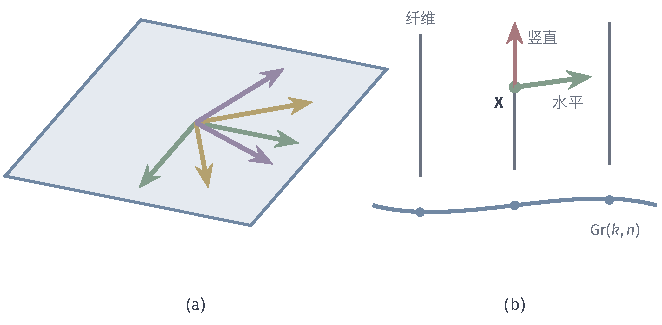
\includegraphics[width=112.0mm]{figures/05-optimization/06-constrained-optimization/tikz/mfo-grassmann-fibre/figure.pdf}
 \caption{子空间的多种表示。(a)~同一平面（浅蓝）的三组标准正交基，绿、黄、紫三组箭头分别对应一种基。(b)~商结构的示意：底部曲线代表$\mathrm{Gr}(k,n)$，每点上方的竖线（纤维）是表示同一子空间的所有$\bm{X}$；红箭头是竖直方向，沿它移动子空间不变，绿箭头是水平方向。}
 \label{fig:mfo-grassmann-fibre}
\end{BookInlineFigure}

\paragraph{竖直方向与水平方向}
沿曲线$\bm{X}\exp(t\bm{\Omega})$（$\bm{\Omega}$反对称）移动，子空间不变，它的速度$\bm{X}\bm{\Omega}$称为竖直方向。与竖直方向正交的切向量满足$\bm{X}^\top\bm{\Delta}=\bm{0}$，它们构成水平空间，每个水平方向都真正改变子空间。

这种分解对梯度有简单的影响。因为$f$沿竖直方向不变，$\operatorname{grad}f$没有竖直分量。由投影公式~\eqref{eq:mfo-stiefel-projection}和$\nabla\bar{f}=\bm{A}\bm{X}$，$\bm{X}^\top\bm{A}\bm{X}$对称，于是
\begin{equation}
 \operatorname{grad}f(\bm{X})=\bm{A}\bm{X}-\bm{X}\bigl(\bm{X}^\top\bm{A}\bm{X}\bigr)=(\bm{I}-\bm{X}\bm{X}^\top)\bm{A}\bm{X}.
 \label{eq:mfo-stiefel-grad}
\end{equation}
满足$\bm{X}^\top\operatorname{grad}f=\bm{0}$，确实是水平的。驻点的条件是$\bm{X}$的列空间是$\bm{A}$的不变子空间。

用贯穿的矩阵算一次。取$\bm{X}=[\bm{x}^{(0)},\bm{E}_1]$，先算
\[
 \bm{X}^\top\bm{A}\bm{X}=\frac19\begin{bmatrix}16&2\\2&25\end{bmatrix},\qquad f(\bm{X})=\frac{41}{18}.
\]

把它代入式~\eqref{eq:mfo-stiefel-grad}，得到
\[
 \operatorname{grad}f(\bm{X})=\frac{1}{27}\begin{bmatrix}-16&-20\\8&10\\16&20\end{bmatrix}.
\]

两列都平行于法向量$\bm{n}=\tfrac13(-2,1,2)^\top$，也就是与平面$\operatorname{span}\bm{X}$垂直的方向。这正好符合水平的要求：要改变一个平面，只能把基朝平面外转动。

取$\alpha=\tfrac12$，先走到$\bm{X}-\tfrac12\operatorname{grad}f(\bm{X})$，然后作回缩。QR回缩与极分解回缩的结果分别是
\[
 \bm{X}^{\mathrm{QR}}\approx\begin{bmatrix}0.8800&0.4504\\0.4738&-0.8549\\0.0338&0.2574\end{bmatrix},\qquad
 \bm{X}^{\mathrm{pol}}\approx\begin{bmatrix}0.8298&0.5373\\0.5580&-0.8025\\0.0076&0.2595\end{bmatrix}.
\]
两者列空间相同，目标值都约为$1.5788$，比原来的$2.2778$小。子空间问题的回缩，只有列空间才有意义，QR分解与极分解的差别不影响目标。

\paragraph{冗余对曲率的影响}
竖直方向对Newton型方法有实质影响。由第~\ref{sec:mfo-optimality}节的做法，Stiefel上的Hessian是
\begin{equation}
 \operatorname{Hess}f(\bm{X})[\bm{\Delta}]=\bm{P}_{\bm{X}}\bigl(\bm{A}\bm{\Delta}-\bm{\Delta}\,\bm{X}^\top\bm{A}\bm{X}\bigr).
 \label{eq:mfo-stiefel-hess}
\end{equation}

取极小点$\bm{X}^\star=[\bm{e}_1,\bm{e}_2]$，此时$\bm{X}^\top\bm{A}\bm{X}$是$\operatorname{diag}(1,2)$，$\mathrm{St}(2,3)$的切空间是$3$维的。取竖直方向$\bm{\Delta}=\bm{X}^\star\bm{\Omega}$，$\bm{\Omega}$是$2\times2$反对称矩阵，代入式~\eqref{eq:mfo-stiefel-hess}算得$\operatorname{Hess}f[\bm{\Delta}]=\bm{0}$，这个方向是零特征方向。

水平方向取$\bm{\Delta}=\bm{e}_3\bm{b}^\top$，算得
\[
 \operatorname{Hess}f[\bm{\Delta}]=\bm{e}_3\,(3b_1,\ 2b_2).
\]
所以$\bm{X}^\star$处Hessian的特征值是$3,2,0$，算子奇异，第~\ref{sec:mfo-newton}节要求的非退化条件在$\mathrm{St}(2,3)$上不成立，而这个零特征值完全是表示引入的。

商结构的办法是把Newton方程限制在水平空间$\bm{X}^\top\bm{\Delta}=\bm{0}$内，这时算子只有$3,2$两个特征值，可逆。实际上就是在$\mathrm{Gr}(k,n)$上计算，但存储仍用矩阵$\bm{X}$。在目标对基变换不变时这样做减少了$k(k-1)/2$个冗余维数。目标若不具备不变性（例如不同列带不同权重），列的次序和基都有意义，就要留在Stiefel流形上。

\paragraph{同一标准下比较}
比较两类方法时，目标、精度和计量单位必须一致，并且要同时报告两个误差。一般约束方法不保证每步可行，只看目标值或只看驻点残差都会误判。下面用问题~\eqref{eq:mfo-subspace-objective}，取$n=200$，$k=5$，$\bm{A}$的特征值在$1$到$100$之间等距。

三种方法都从同一个随机起点出发。黎曼梯度下降和黎曼信赖域使用QR回缩，后者在Grassmann结构上运行。第~\ref{chap:penalty-multiplier-methods}章的增广Lagrange方法用有限记忆拟Newton法解内层问题，迭代中不做回缩。残差统一在当前点作QR所得的$\bm{Q}$上计算，以便不同方法使用同一标准：
\[
 \lVert(\bm{I}-\bm{Q}\bm{Q}^\top)\bm{A}\bm{Q}\rVert_{\mathrm{F}}.
\]

结果见图~\ref{fig:mfo-method-compare}和表~\ref{tab:mfo-method-results}。计量单位是$\bm{A}$乘一列向量的次数。增广Lagrange在迭代中途离开可行集，可行误差最大约为$1.66$，随外层更新才回到机器精度，这时已经用了$10^5$量级的乘积。两种流形方法每一步都保持机器精度的可行性。

\begin{BookInlineFigure}
 \centering
 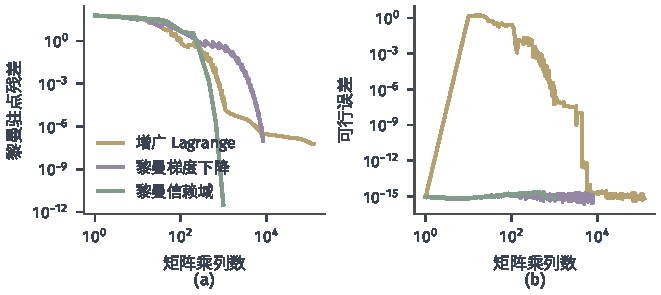
\includegraphics[width=112.0mm]{figures/05-optimization/06-constrained-optimization/matplotlib/mfo-method-compare/figure.pdf}
 \caption{$\mathrm{St}(5,200)$上的子空间问题，横轴是$\bm{A}$乘列向量的累计次数。黄线为增广Lagrange方法，紫线为黎曼梯度下降，绿线为黎曼信赖域。(a)~黎曼驻点残差。(b)~可行误差$\lVert\bm{X}^\top\bm{X}-\bm{I}\rVert_{\mathrm{F}}$。这是单个问题实例的一次运行，三种方法都未作专门调参。}
 \label{fig:mfo-method-compare}
\end{BookInlineFigure}

\begin{BookInlineTable}
 \centering
 \caption{图~\ref{fig:mfo-method-compare}的运行结果，三种方法的黎曼驻点残差的容差均为$10^{-7}$。}
 \label{tab:mfo-method-results}
 \begin{tabular}{lllll}
  \toprule
  方法 & 乘列数 & QR次数 & 驻点残差 & 最大可行误差\\
  \midrule
  增广Lagrange & $123560$ & $0$ & $5.9\times10^{-8}$ & $1.66$\\
  黎曼梯度下降 & $8110$ & $3244$ & $9.9\times10^{-8}$ & $2.4\times10^{-15}$\\
  黎曼信赖域 & $980$ & $11$ & $3.4\times10^{-12}$ & $2.3\times10^{-15}$\\
  \bottomrule
 \end{tabular}
\end{BookInlineTable}

计量也要诚实。这个问题的$\bm{A}$是对角阵，乘一列只要$200$次运算，一次$n\times k$矩阵的QR约需$nk^2=5000$次。按此换算，黎曼梯度下降的主要代价其实是回缩：回溯的每次试探都做一次QR，$3244$次QR约$1.6\times10^7$次运算，比矩阵乘积的$1.6\times10^6$次多一个数量级。若$\bm{A}$的乘积昂贵，结论又会不同。

表~\ref{tab:mfo-cost-compare}按运算种类汇总。流形方法的优势依赖一个前提：回缩、投影和搬运有便宜的闭式。这对球面和正交矩阵成立，对一般的非线性等式约束不成立，回缩本身可能要解一个非线性方程，这时第~\ref{chap:feasible-iterations}章的恢复步或第~\ref{chap:sequential-quadratic-programming}章的SQP未必更差。可行集带不等式或棱角时，本章方法也不适用。

\begin{BookInlineTable}
 \centering
 \caption{一般约束方法与流形方法的每轮运算对比，$\mathrm{St}(k,n)$上的问题。}
 \label{tab:mfo-cost-compare}
 \begin{tabular}{lll}
  \toprule
  项目 & 一般约束方法 & 流形方法\\
  \midrule
  导数 & $\nabla\bar{f}$，约束Jacobian & $\nabla\bar{f}$，再作投影$O(nk^2)$\\
  线性求解 & KKT系统，维数$nk+k(k+1)/2$ & 切空间内，维数$\dim M$\\
  保持可行 & 外层逐步逼近，或恢复步 & 回缩，$O(nk^2)$\\
  比较历史 & 同一空间，直接相减 & 需要搬运\\
  \bottomrule
 \end{tabular}
\end{BookInlineTable}

\paragraph{报告什么}
无论采用哪种方法，收尾时都要给出同样的两项：可行误差$\lVert h(\bm{x})\rVert$与黎曼驻点残差$\lVert\operatorname{grad}f(\bm{x})\rVert$。流形方法的可行误差应当是机器精度量级，若它随迭代缓慢增长，说明回缩或投影累积了舍入误差，需要定期重新正交化。
